\section{Results and Discussion}
\label{results}

%As discussed before, diagnosing malaria involves 5 different steps to be performanced. In this paper, we propose a deep learning architecture to be use both in the background separation and sample classification step.

In this section, we present our results regarding the deep learning architecture proposed in Section \ref{segmethod}, with focus on the problem of separation of background objects from the blood smear. Figs. \ref{fig:gen50},\ref{fig:gen250} and \ref{fig:gen30410} present samples of images generated after 50, 250 and 30410 epochs, respectively, by the DCGAN network.  

\begin{figure}[h]
\caption{Generated images after 50 epochs}
\label{fig:gen50}
\begin{center}
\includegraphics[scale=0.45]{./images/generation/alta_mnist_50.png} \end{center}
\end{figure}

\begin{figure}[h]
\caption{Generated images after 250 epochs}
\label{fig:gen250}
\begin{center}
\includegraphics[scale=0.45]{./images/generation/alta_mnist_250.png} \end{center}
\end{figure}

\begin{figure}[h]
\caption{Generated images after 30410 epochs}
\label{fig:gen30410}
\begin{center}
\includegraphics[scale=0.45]{./images/generation/alta_mnist_30410.png} \end{center}
\end{figure}

%\begin{figure*}[htp]
%  \label{fig:threshold}
%  \centering
%  \subfigure[Blood smears image with Adaptive Thresholding]{
%  %\caption{Generated images after 30410 epochs}
%  %\label{fig:threshold}
%  \includegraphics[scale=0.21]{./images/threshold.png}
%  }
%  \subfigure[Blood smears image with object detection]{
%  %\caption{Generated images after 30410 epochs}
%  %\label{fig:objectdetect}
%  \includegraphics[scale=0.25]{./images/object_detected.png}
%  }
%\end{figure*}

%Those images were used to train the CNN network. Table \ref{tab:results} presents the results for eight executions. The CNN network was trained with generated images and tested with real images. With 2200 generated images by the DCGAN network, the CNN network obtain 100\% of accuracy with the real images. From the results presented in the experiments, we observe that the images generated by the DCGAN network can be used in the training of a CNN network to detect objects improving classifier accuracy.

%\input{tables/tableResult.tex}

%Finally, Fig. \ref{fig:threshold} - (b) shows samples of objects detected by the proposed process.  The bounding boxes presented correspond to objects separated from the background of the exam.

%Despite the high accuracy obtained in the tests applied in the set of 600 test images used, this process corresponds to only part of the problem of automated malaria diagnosis. There is a second challenge of choosing the best regions to be classified in the blood smear obtained. Future approaches such as the use of YOLO or Region Based CNN may present better results. 
The diagnosis of malaria still depends on the development of a classifier that performs the classification of the objects extracted from the examination. 
%ALLBERSON TIROU 29/11/2018 - As in this work we attend to show the use of samples generated by GAN networks in order to enhance the performance of an CNN classifier. 
In order to present some empirical evidence of our claim, we used only the images generated by the GAN network to train a CNN classifier. In the following, we report the results of such experiments, as well as, we lay down some considerations and comments on the results.

We consider 3 of the most famous metrics in the field of machine learning to evaluate the efficiency of our approach. Those metrics are: precision, recall and f1-score. 

\begin{figure}[h]
\caption{Report on the precision}
\label{fig:precision}
\begin{center}
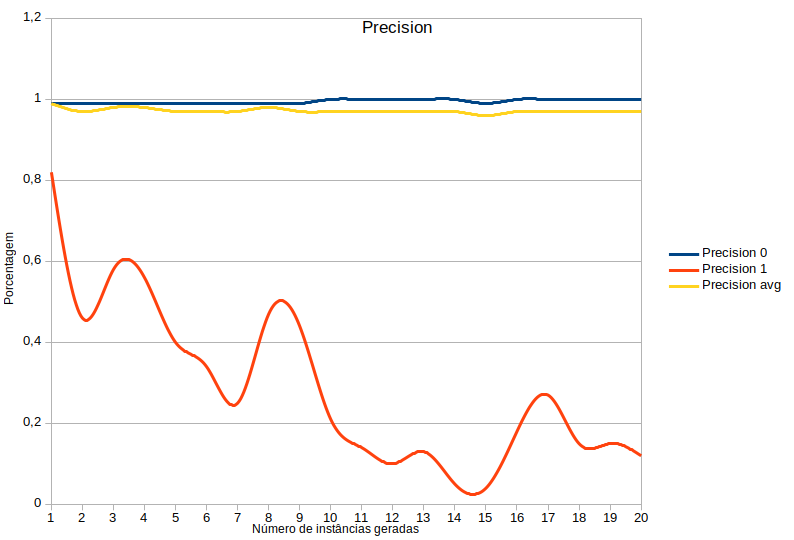
\includegraphics[scale=0.40]{./images/figura1.png} \end{center}
\end{figure}

In Figure~\ref{fig:precision}, we present the results concerning the precision. In the x-axis we have the number of instances in thousands, the y-axis represents the precision score for each class (class 0, that represents the background and class 1, that represents the plasmodium samples) and the average precision. Notice that the average precision and the class 1 precision are quite steady and quite high as we claimed. Although, as we can see the precision is decreasing for the class 1, we believe that this is due to the overfitting generated by the larger number of samples in the class 0. 

\begin{figure}[h]
\caption{Report on the recall}
\label{fig:recall}
\begin{center}
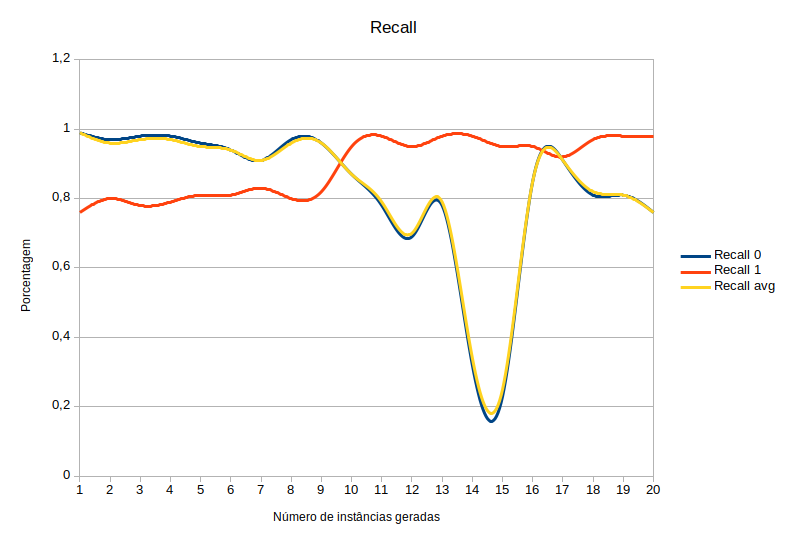
\includegraphics[scale=0.40]{./images/figura2.png} \end{center}
\end{figure}

In Figure~\ref{fig:recall}, the results concerning the recall are shown. In the x-axis we have the number of instances in thousands, the y-axis depicts the recall score for each class (class 0, representing the background and class 1, representing the plasmodium samples) and the average recall. Observe that the average recall is also quite steady and that the recall suffers the same problem of the precision due to overfitting.

\begin{figure}[h]
\caption{Report on the f1-score}
\label{fig:f1score}
\begin{center}
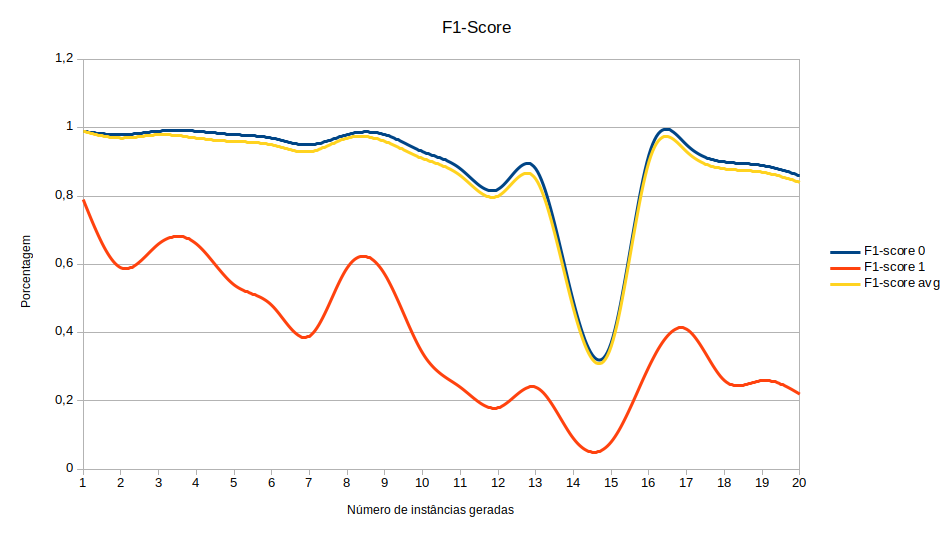
\includegraphics[scale=0.40]{./images/figura3.png} \end{center}
\end{figure}

 Finally, we present in Figure~\ref{fig:f1score} the results related to the f1-score. Again, in the x-axis we show the number of instances in thousands, the y-axis contains the f1-score score for each class (class 0, that represents the background and class 1, that represents the plasmodium samples) and the average f1-score. 




We reinforce that, as we claimed, the use of the generated samples alone are responsible for a good accuracy in the proposed CNN network model, and this process corresponds to only part of the problem of automated malaria diagnosis. There is a second challenge of choosing the best regions to be classified in the blood smear obtained. Future approaches, such as the use of YOLO or Region Based CNN, may present better results. Nevertheless, the recall and specially the f1-score tend to increase with the number of generated samples. Such behavior shows us that a fine tune is need to be able to use the generated images without loosing performance. 